
%(BEGIN_QUESTION)
% Copyright 2010, Tony R. Kuphaldt, released under the Creative Commons Attribution License (v 1.0)
% This means you may do almost anything with this work of mine, so long as you give me proper credit

Examine this switch circuit and determine what process condition(s) must be met in order to turn the lamp on:

$$\includegraphics[width=15.5cm]{i02227x01.eps}$$

\vfil 

\underbar{file i02227}
\eject
%(END_QUESTION)





%(BEGIN_ANSWER)

This is a graded question -- no answers or hints given!

%(END_ANSWER)





%(BEGIN_NOTES)

This is an example of a problem where re-drawing the circuit in schematic form makes it easier to understand:

$$\includegraphics[width=15.5cm]{i02227x02.eps}$$

In order to energize the lamp, the pressure switch must be closed, and either the temperature switch or the level switch must also be closed.  We know that the temperature and level conditions necessary to energize the lamp are an ``OR'' logical function because those two switches are wired in parallel with each other: only one of them has to close in order to pass electric current to the lamp.  The pressure switch, however, is wired in series with the lamp and so its condition is a {\it necessity} for closing the lamp circuit.

\vskip 10pt

For any normally-closed (NC) switch, this means the stimulus must be {\it less than} the threshold value in order to make it close.  For any normally-open (NO) switch, this means the stimulus must be {\it greater than} the threshold value in order to make it close. 

\vskip 10pt

$P <$ 33 PSI {\bf and} ($T >$ 141 $^{o}$F {\bf or} $L <$ 2.3 ft).

%INDEX% Pictorial circuit review (process switch circuit)
%INDEX% Switch, ``normal'' status

%(END_NOTES)


